\section{Compression Factor Studies}

For studies in this article, we used compression factor 4, where the input data with 48 values was compressed into a latent space vector of length 12. However, the 
latent space vector can be changed to a smaller value to achieve a higher compression factor, but the resolution of the reconstructed pulse integral deteriorates as 
a function of the compression level. The following studies were done using a latent space layer set to 24, 8 and 6 lengths, increasing the compression ratio to 2, 6 and 8 respectively.

\begin{figure}[h!]
\centering
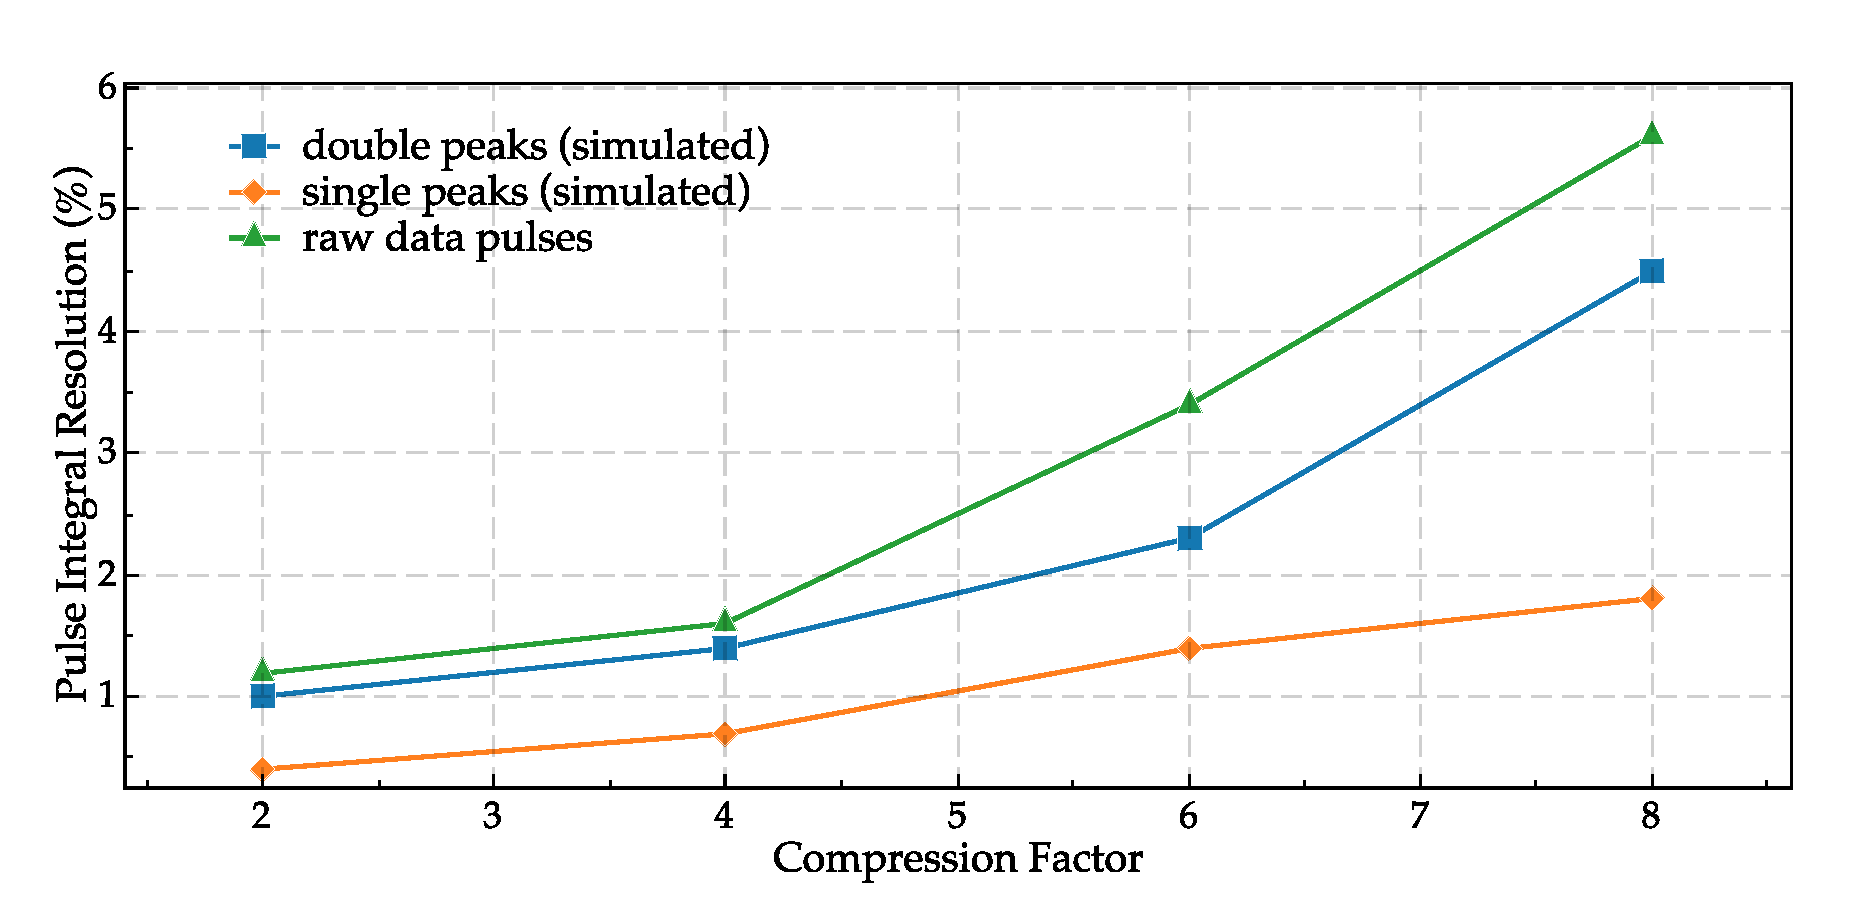
\includegraphics[width=0.95\columnwidth]{cfactor_summary.pdf}
\caption{The resolution of decompressed pulse integral as a function of compression factor.} 
\label{fig:compression_factor_summary}
\end{figure}

The result for three different data sets are shown in Figure~\ref{fig:compression_factor_summary}, the resolution decrease in single peak simulated data is linear and decreases with the increased compression ratio. In the double peak simulated and raw data the decoded peak resolution decreases rapidly with the compression ratio increase, reaching above $5\%$ for the compression ratio of 8.
The studied neural network (autoencoder) is capable of compression pulses into much smaller latent space and preserves very well the position of the peak but has some resolution depending on the compression ratio. Depending on the requirements of the situation different compression ratios can be used.
